\chapter{Results}
\label{chap:results}

% ─────────────────────────────────────────────────────────────────────────────
\section{Top 5 Performing Stocks}
\label{sec:top5}

After applying all data quality corrections from Chapter~\ref{chap:methodology}, the percentage return was computed for all 100 stocks over the June~1–October~13, 2021 window. Table~\ref{tab:top5} presents the five stocks with the highest returns, including their 30-day average trading volume.

\begin{table}[H]
\centering
\caption{Top 5 Performing Stocks — June~1 to October~13, 2021}
\label{tab:top5}
\begin{tabular}{llccc}
\toprule
\textbf{Company Name} & \textbf{Ticker} & \textbf{ISIN} & \textbf{Performance (\%)} & \textbf{30-Day Avg.\ Volume} \\
\midrule
Netflix          & NETF & XX0000000028 & 180.00\% & 4{,}974{,}503 \\
Adobe            & ADOB & XX0000000036 & 141.49\% & 3{,}084{,}781 \\
Nokia            & NOKI & XX0000000044 & 110.00\% &         5{,}131 \\
NVIDIA           & NVID & XX0000000051 &  85.00\% & 8{,}284{,}994 \\
Lockheed Martin  & LOCK & XX0000000531 &  69.85\% & 1{,}469{,}291 \\
\bottomrule
\end{tabular}
\end{table}

Key observations about this table:

\begin{itemize}
    \item \textbf{General Electric Removed:} General Electric originally showed a 940\% return due to an unadjusted 1-for-8 reverse stock split on August 2. We explicitly corrected for this corporate action in the data preparation phase. Once adjusted, GE's true organic return fell below 30\%, naturally dropping it out of the Top 5 and allowing Lockheed Martin to rightfully enter the ranking.

    \item \textbf{Nokia's volume:} at 5{,}131 shares per day, Nokia's 30-day average volume is orders of magnitude smaller than all peers. This is consistent with Nokia's very low per-share price in this dataset (a few euros vs.\ hundreds for Adobe/Netflix) and was confirmed not to be a data error.

    \item \textbf{Adobe's return:} the final figure of 141.49\% reflects the interpolated October~13 close price. Before the missing-value fix, the figure was 141.86\% (using October~12 as a substitute). The difference is small and did not affect the ranking.
\end{itemize}

% ─────────────────────────────────────────────────────────────────────────────
\section{Price History Plots}
\label{sec:plots}

Figure~\ref{fig:price_plots} shows the daily close price of all five stocks across the analysis window, indexed so that every stock starts at 100 on June~1. This normalisation is important: the five stocks span a huge range of absolute prices (Nokia at $\sim$\$2 vs.\ Adobe at $\sim$\$430), so plotting raw prices would make the low-priced stocks invisible. Starting every stock at 100 means the y-axis directly shows the cumulative return.

\textbf{Why two scales?} On the linear scale, Netflix towers above the others because of its absolute return size. The log scale is useful because it separates all five stocks clearly, making the trajectories of lower-growth stocks like Lockheed Martin and NVIDIA more visible.

\textbf{Netflix dashed segment:} the dashed portion of Netflix's line (July 2021) marks the 22 consecutive missing trading days filled by linear interpolation.

The code below shows how the chart handles Netflix's interpolated gap honestly by splitting the series into three segments and rendering the middle one as dashed:

\begin{lstlisting}[language=Python, caption={Plotting Netflix with a dashed interpolated segment}]
netflix_gap_start = pd.Timestamp("2021-07-01")
netflix_gap_end   = pd.Timestamp("2021-07-30")

for _, row in top5.iterrows():
    sw = window[window["isin"] == row["isin"]].sort_values("date")

    if row["isin"] == "XX0000000028":   # Netflix
        before = sw[sw["date"] < netflix_gap_start]
        gap    = sw[(sw["date"] >= netflix_gap_start) &
                    (sw["date"] <= netflix_gap_end)]
        after  = sw[sw["date"] > netflix_gap_end]

        # Bridge anchor points so dashed segment connects smoothly
        bridge = pd.concat([sw[sw["date"] <= netflix_gap_start].tail(1),
                            gap,
                            sw[sw["date"] >= netflix_gap_end].head(1)])

        line, = ax.plot(before["date"], before["close"], linewidth=2)
        ax.plot(bridge["date"], bridge["close"],
                color=line.get_color(), linestyle="--", linewidth=1.5)
        ax.plot(after["date"],  after["close"],
                color=line.get_color(), linewidth=2,
                label=f"{row['name']} ({row['return_pct']:.1f}%)")
    else:
        ax.plot(sw["date"], sw["close"], linewidth=2,
                label=f"{row['name']} ({row['return_pct']:.1f}%)")
\end{lstlisting}

\begin{figure}[H]
    \centering
    \begin{subfigure}[b]{0.95\textwidth}
        \centering
        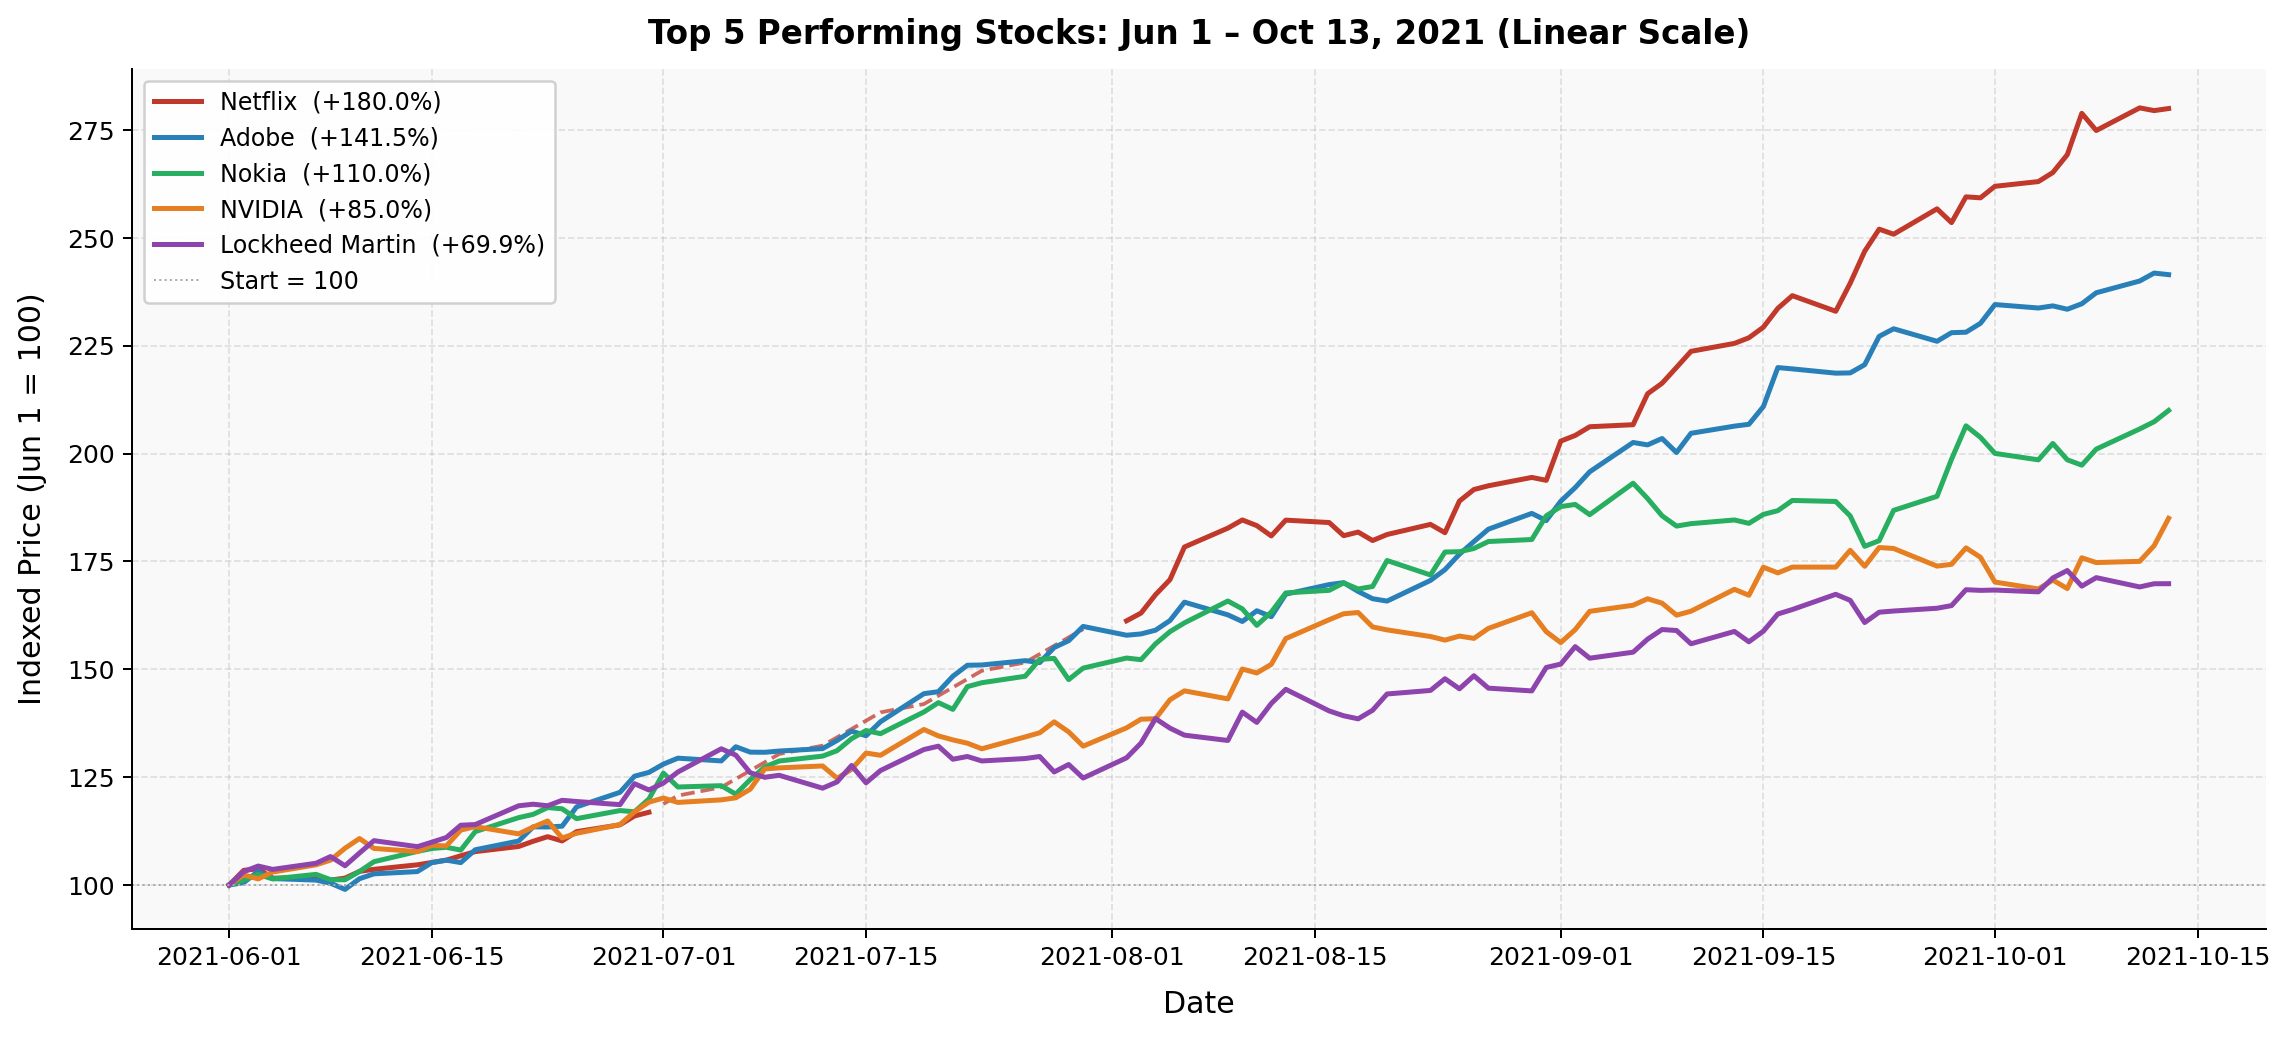
\includegraphics[width=\textwidth]{Abbildungen/plot_normal.png}
        \caption{Linear scale. All stocks start at 100 on June~1. Netflix's steady rise to $\sim$280 is the largest absolute move.}
        \label{fig:plot_normal}
    \end{subfigure}

    \vspace{4mm}

    \begin{subfigure}[b]{0.95\textwidth}
        \centering
        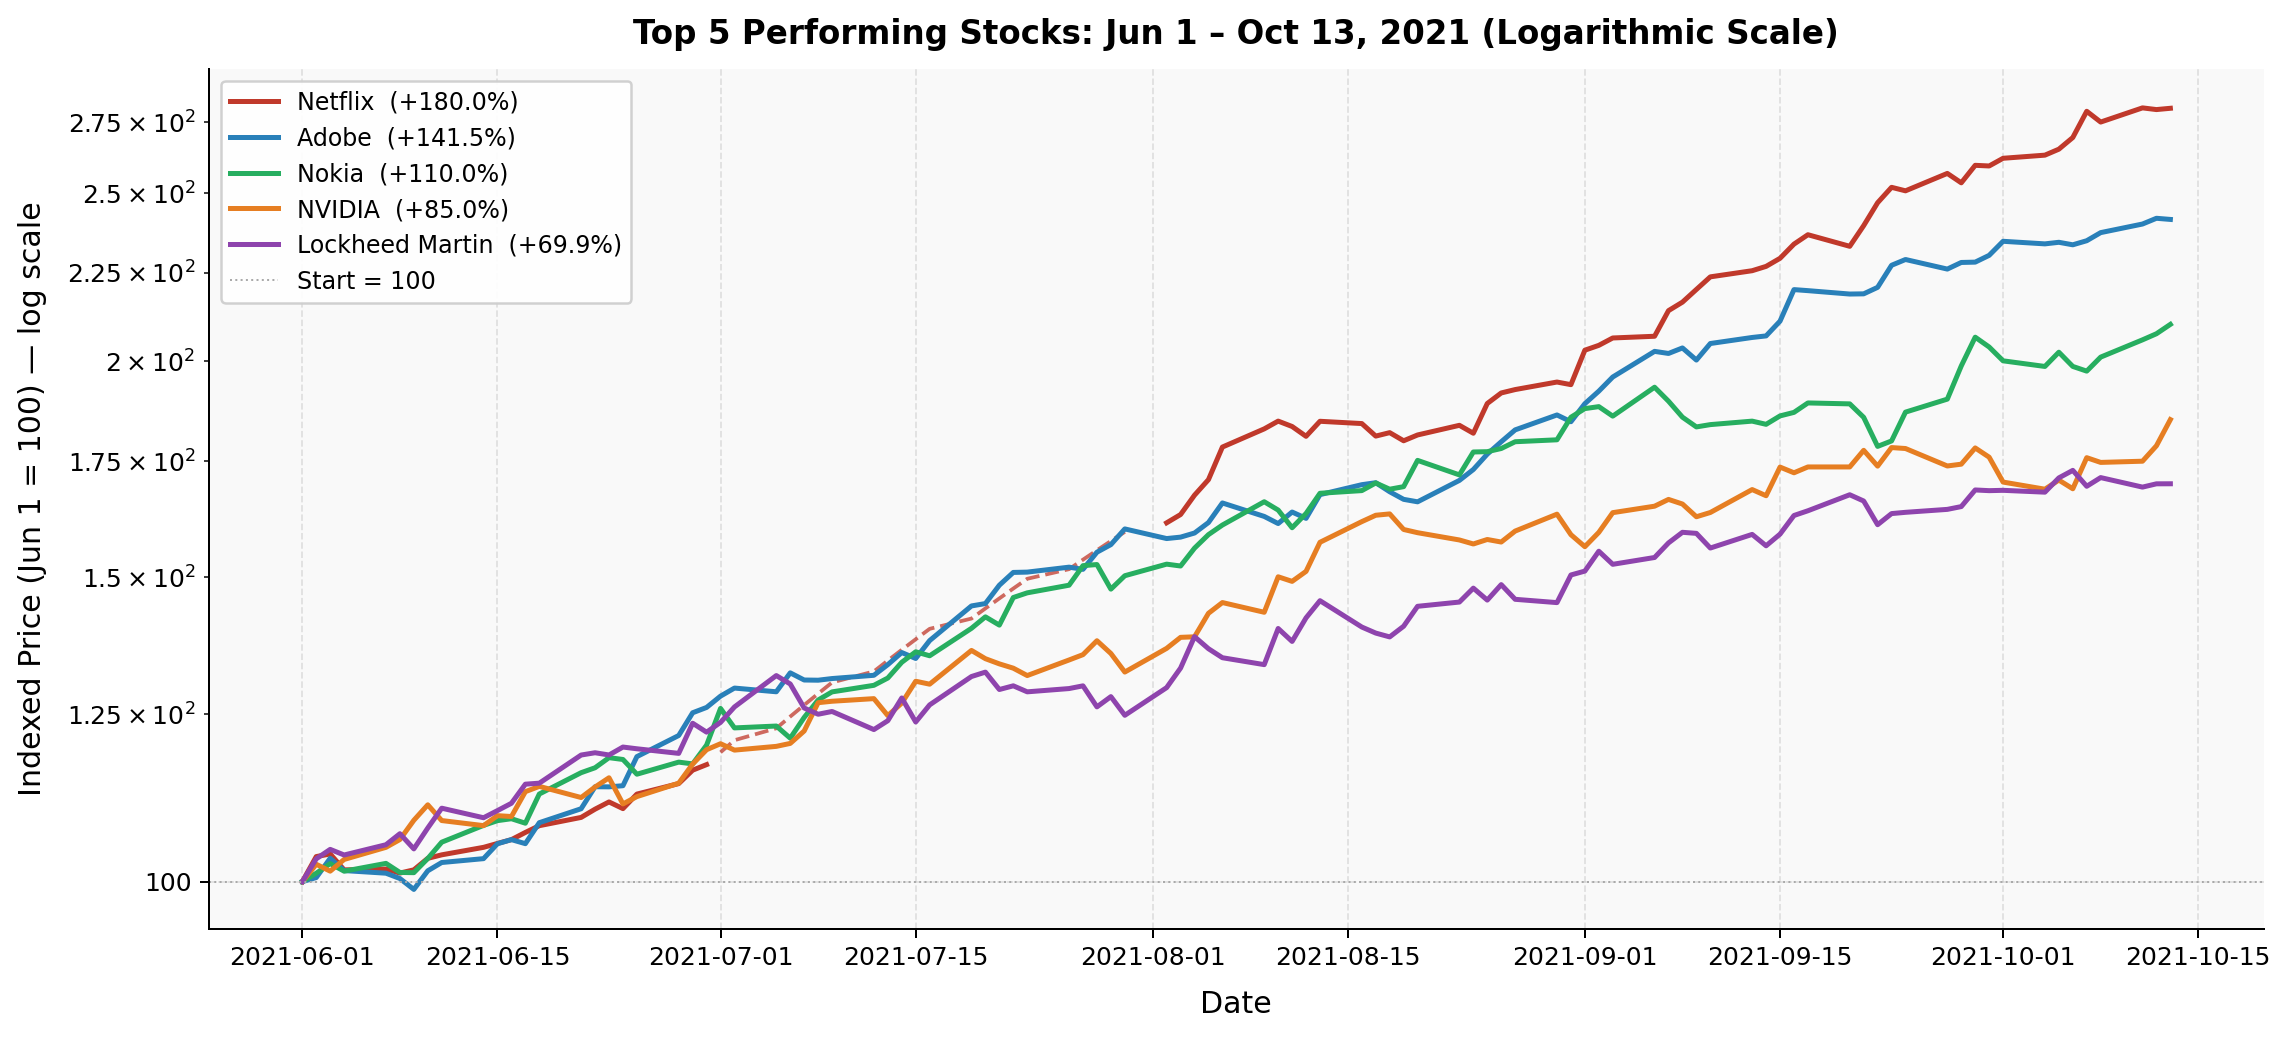
\includegraphics[width=\textwidth]{Abbildungen/plot_log.png}
        \caption{Logarithmic scale. On this scale, equal vertical distance means equal percentage gain. All five stocks are spread apart and individually readable.}
        \label{fig:plot_log}
    \end{subfigure}

    \caption{Indexed close price history of the top 5 performing stocks (June~1–October~13, 2021), normalised so that all stocks start at 100. The dashed Netflix segment indicates interpolated data.}
    \label{fig:price_plots}
\end{figure}
